%\documentclass[handout]{ximera}
\documentclass[nooutcomes]{ximera}

\usepackage{gensymb}
\usepackage{tabularx}
\usepackage{mdframed}
\usepackage{pdfpages}
%\usepackage{chngcntr}

\let\problem\relax
\let\endproblem\relax

\newcommand{\property}[2]{#1#2}




\newtheoremstyle{SlantTheorem}{\topsep}{\fill}%%% space between body and thm
 {\slshape}                      %%% Thm body font
 {}                              %%% Indent amount (empty = no indent)
 {\bfseries\sffamily}            %%% Thm head font
 {}                              %%% Punctuation after thm head
 {3ex}                           %%% Space after thm head
 {\thmname{#1}\thmnumber{ #2}\thmnote{ \bfseries(#3)}} %%% Thm head spec
\theoremstyle{SlantTheorem}
\newtheorem{problem}{Problem}[]

%\counterwithin*{problem}{section}



%%%%%%%%%%%%%%%%%%%%%%%%%%%%Jenny's code%%%%%%%%%%%%%%%%%%%%

%%% Solution environment
%\newenvironment{solution}{
%\ifhandout\setbox0\vbox\bgroup\else
%\begin{trivlist}\item[\hskip \labelsep\small\itshape\bfseries Solution\hspace{2ex}]
%\par\noindent\upshape\small
%\fi}
%{\ifhandout\egroup\else
%\end{trivlist}
%\fi}
%
%
%%% instructorIntro environment
%\ifhandout
%\newenvironment{instructorIntro}[1][false]%
%{%
%\def\givenatend{\boolean{#1}}\ifthenelse{\boolean{#1}}{\begin{trivlist}\item}{\setbox0\vbox\bgroup}{}
%}
%{%
%\ifthenelse{\givenatend}{\end{trivlist}}{\egroup}{}
%}
%\else
%\newenvironment{instructorIntro}[1][false]%
%{%
%  \ifthenelse{\boolean{#1}}{\begin{trivlist}\item[\hskip \labelsep\bfseries Instructor Notes:\hspace{2ex}]}
%{\begin{trivlist}\item[\hskip \labelsep\bfseries Instructor Notes:\hspace{2ex}]}
%{}
%}
%% %% line at the bottom} 
%{\end{trivlist}\par\addvspace{.5ex}\nobreak\noindent\hung} 
%\fi
%
%


\let\instructorNotes\relax
\let\endinstructorNotes\relax
%%% instructorNotes environment
\ifhandout
\newenvironment{instructorNotes}[1][false]%
{%
\def\givenatend{\boolean{#1}}\ifthenelse{\boolean{#1}}{\begin{trivlist}\item}{\setbox0\vbox\bgroup}{}
}
{%
\ifthenelse{\givenatend}{\end{trivlist}}{\egroup}{}
}
\else
\newenvironment{instructorNotes}[1][false]%
{%
  \ifthenelse{\boolean{#1}}{\begin{trivlist}\item[\hskip \labelsep\bfseries {\Large Instructor Notes: \\} \hspace{\textwidth} ]}
{\begin{trivlist}\item[\hskip \labelsep\bfseries {\Large Instructor Notes: \\} \hspace{\textwidth} ]}
{}
}
{\end{trivlist}}
\fi


%% Suggested Timing
\newcommand{\timing}[1]{{\bf Suggested Timing: \hspace{2ex}} #1}




\hypersetup{
    colorlinks=true,       % false: boxed links; true: colored links
    linkcolor=blue,          % color of internal links (change box color with linkbordercolor)
    citecolor=green,        % color of links to bibliography
    filecolor=magenta,      % color of file links
    urlcolor=cyan           % color of external links
}

\title{Side-Splitter Theorems}
\author{Bart Snapp and Brad Findell}

\outcome{Learning outcome goes here.}

\begin{document}
\begin{abstract}
  We prove a basic theorem about similar triangles.
\end{abstract}
\maketitle

\begin{teachingnote}
\end{teachingnote}

In this activity, we will show that the properties of dilations, which you noticed in a previous activity, can be proven \emph{without} using facts about transversals and parallel lines.  Instead, we use the area formulas for rectangles, triangles, and 
parallelograms.  \emph{Note: For a given base, draw the corresponding altitude to reason about a triangle's area.}
\begin{question}
What must be true about the base and height measurements for these area formulas to be valid?
\end{question}
%\QM

\begin{problem}
If the area of $\triangle SPR = 8$ square inches and the area of $\triangle QPR = 5$ square inches, then what can you say about $\frac{SR}{RQ}$?  What about $\frac{SR}{SQ}$?  What can you say generally about how these ratios depend upon the areas of the triangles?  
\begin{image}
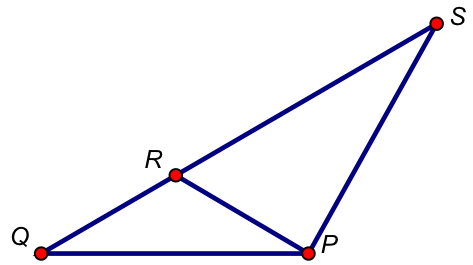
\includegraphics[scale=0.65]{sideSplitter1}
\end{image}
\end{problem}

\begin{problem}
For the trapezoid below, explain why the area of $\triangle BAD$ is equal to the area of $\triangle BAC$.  Name two other triangles that have the same area.
\begin{image}
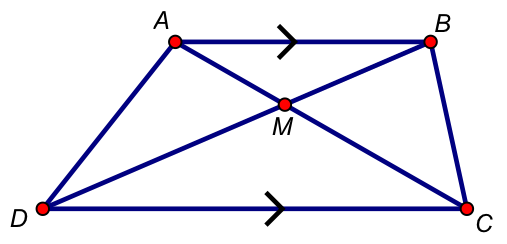
\includegraphics[scale=0.65]{sideSplitter2}
\end{image}
\end{problem}

\begin{problem}
For the parallelogram below, which triangle has the greatest area: $\triangle XYZ$, $\triangle WXY$, $\triangle ZWX$, or $\triangle YZW$?  Explain.  
\begin{image}
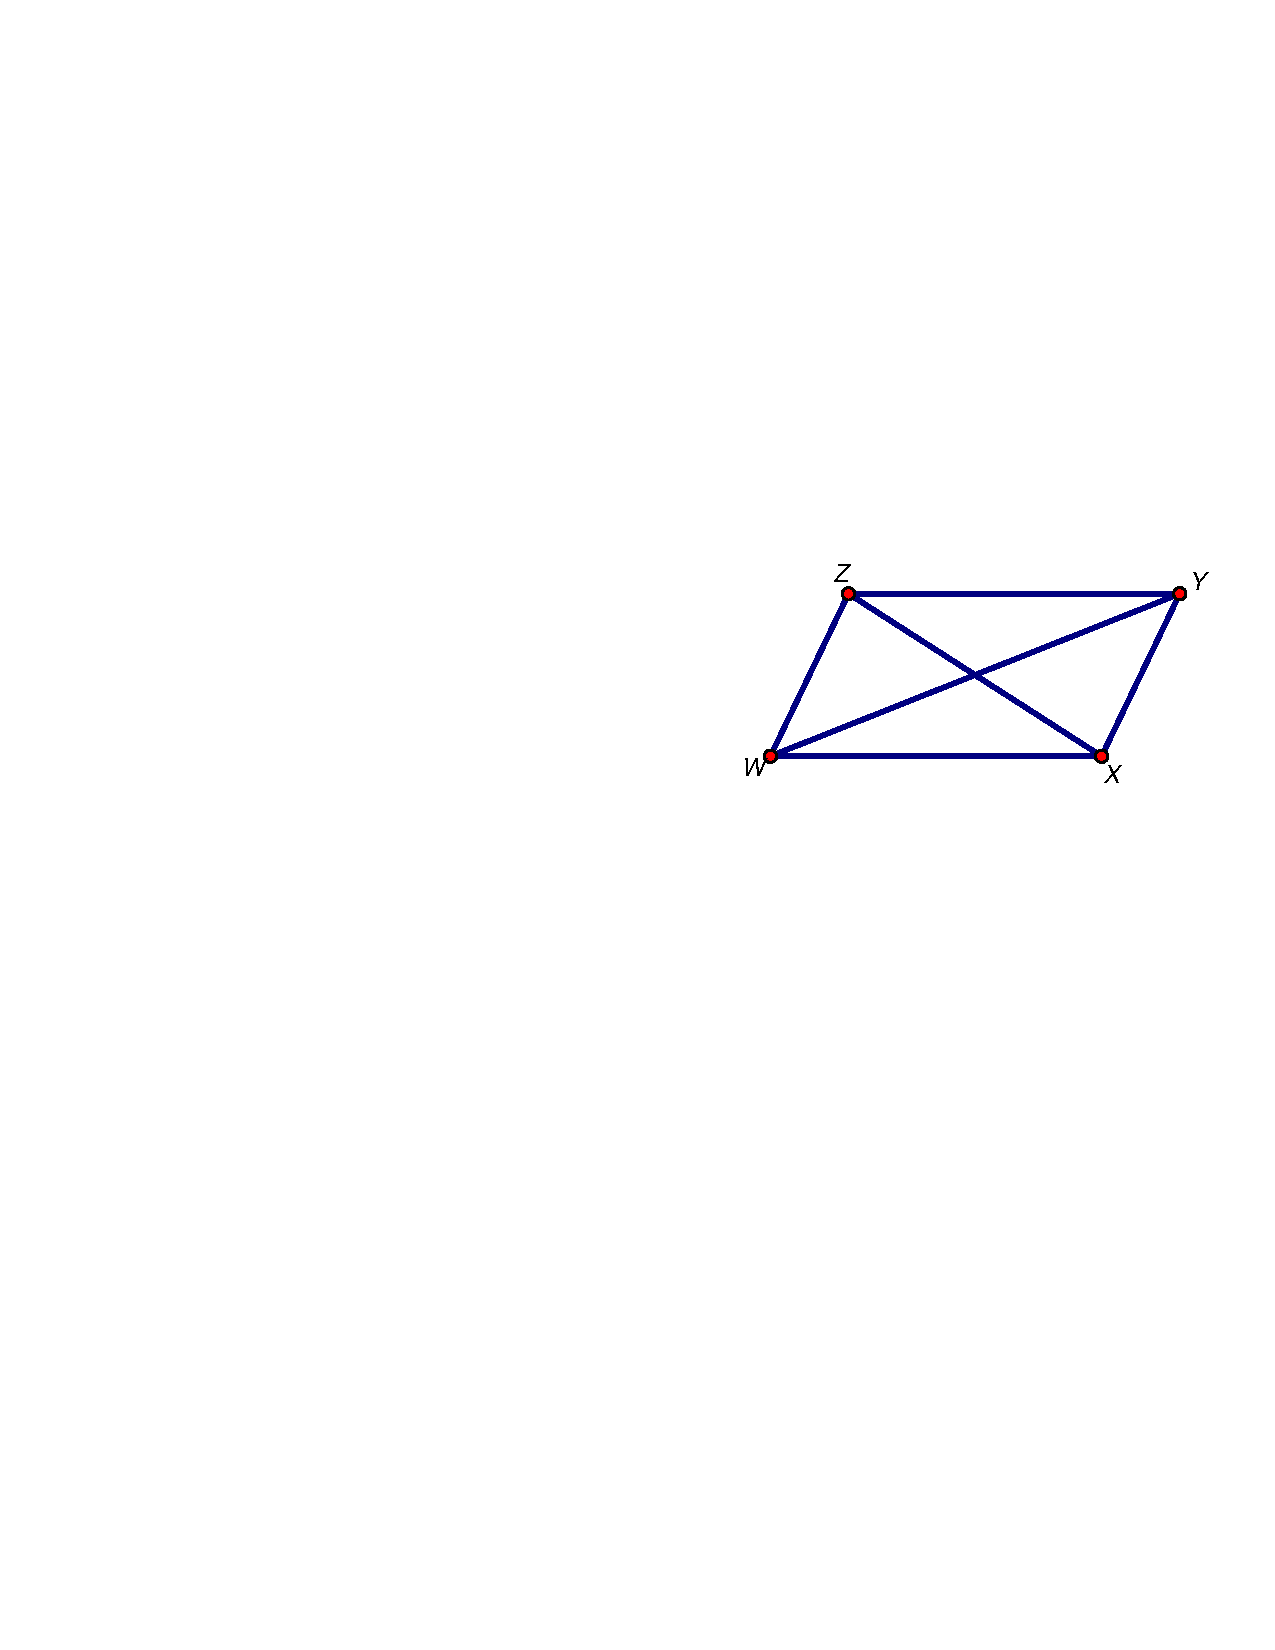
\includegraphics[scale=0.65]{sideSplitter3}
\end{image}
\end{problem}

\begin{teachingnote}
An important objective in the next two problems is the habit of using an equation string, one modification at a time, to show that two expressions are equivalent.
\end{teachingnote}

\begin{problem}
Prove the \textbf{Parallel-Side Theorem}:  If a line in a triangle is parallel to a side of a triangle, then it splits the other sides of the triangle proportionally. 
\begin{image}
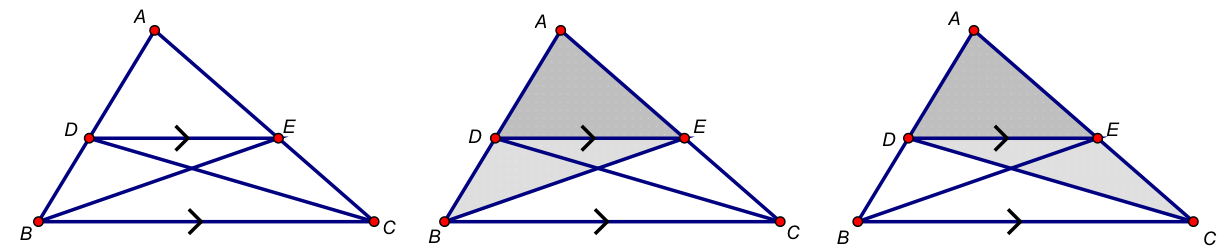
\includegraphics[scale=0.8]{sideSplitter4}
\end{image}
\begin{enumerate}
\item How do the areas of $\triangle ADE$ and $\triangle DBE$ relate to $AD$ and $DB$?  Explain.  
\item How do the areas of $\triangle ADE$ and $\triangle ECD$ relate to $AE$ and $EC$?  Explain. 
\item How do the areas of $\triangle DBE$ and $\triangle ECD$ compare?  Explain.  
\item Use the previous results to show that $\frac{DB}{AD} = \frac{EC}{AE}$.  
\item What the heck did we just do?  What does this say?
\item Where in the proof did we use the fact that $\overline{DE} \parallel \overline{BC}$?  
\end{enumerate}
\end{problem}

\begin{teachingnote}
In the following argument, the triangles refer to their areas.  
Two pairs of triangles with the same height and different bases:  
\[
\frac{DB}{AD} = \frac{\triangle DBE}{\triangle ADE}
\]
\[
\frac{EC}{AE} = \frac{\triangle ECD}{\triangle ADE}
\]
Because of the parallel lines, a pair of triangles with the same height and the same base:  
\[
\triangle DBE = \triangle ECD
\]
Putting this together, we have:  
\[
\frac{DB}{AD} = \frac{\triangle DBE}{\triangle ADE} = \frac{\triangle ECD}{\triangle ADE}
=\frac{EC}{AE}
\]
\end{teachingnote}


\begin{problem}
Use some algebra to show, in the previous picture, that $\frac{AB}{AD} = \frac{AC}{AE}$.
\end{problem}

\begin{teachingnote}
\[
\frac{AB}{AD} = \frac{AD+DB}{AD} = 1 + \frac{DB}{AD} =  1 + \frac{EC}{AE} 
= \frac{AE + EC}{AE} = \frac{AC}{AE}
\]
\end{teachingnote}

\begin{problem}
Prove:  Next we prove, in the previous figure, that $ \frac{BC}{DE} = \frac{AB}{AD} = \frac{AC}{AE}$.  Here are the steps.  
\begin{enumerate}
\item How do we know that $\angle ADE \cong \angle ABC$?  
\item Translate $\triangle ADE$ by the vector $\overrightarrow{DB}$ so that the image $\angle A'D'E'$ of $\angle ADE$ coincides with $\angle ABC$.  Draw a picture of the result.  
\item What segments are parallel now?  How do you know?  
\item Now explain why $\frac{BC}{DE} = \frac{AB}{AD} = \frac{AC}{AE}$ is equal to a common ratio from the previous problem.  
\end{enumerate}
\end{problem}

\begin{problem}
Explain briefly how the Parallel-Side Theorem implies the AA criterion for triangle similarity.  (Hint: Be sure to use the definition of similarity in terms of basic rigid motions and dilations.)  
% Hint:  You need to begin with two triangles that have two pairs of congrent angles.  You need to show (generally) that there exists a sequence of basic rigid motions and dilations that maps one triangle onto the other.  Be sure to consider how you would know whether a reflection is needed as one of the basic rigid motions.  
\end{problem}

\begin{problem}
The \textbf{Split-Side Theorem} is the converse of the Parallel-Side Theorem.   
\begin{enumerate}
\item State the Split-Side Theorem.   
% If a line in a triangle splits two sides proportionally, then it is parallel to the third side of the triangle.
\item Prove the Split-Side Theorem.  (Hint:  Using the previous figures, draw a line through $D$ and parallel to $\overline{BC}$, and let $X$ be the point where the new line intersects $\overline{AC}$.  By the previous results, $\overline{DX}$ divides the sides proportionally.  Then argue that $E$ and $X$ must be the same point.)  
\end{enumerate}
\end{problem}



\begin{problem}
Use the Split-Side Theorem to justify the following properties of a dilation given by a center and a scale factor:
\begin{enumerate}
\item A dilation takes a line not passing through the center of the dilation to a parallel line, and leaves a line passing through the center unchanged.
\item The dilation of a line segment is longer or shorter in the ratio given by the scale factor.
\end{enumerate}
% Hint: You need to begin with a dilation, and you need to show that it has the listed properties.  In addition to the Split-Side Theorem, you may also use other results established in this activity. 

\end{problem}

\begin{problem}
Explain briefly how the Split-Side Theorem establishes the SAS criterion for triangle similarity.  
\end{problem}


\end{document}
